% answers.tex —— 2006 年·普通高等学校招生考试·天津卷文科 · 参考答案与详细解析片段
% 由 tools/generate_projects.py 依来源总账自 2006/2006_数学真题_天津文_试题.md + 2006/2006_数学真题_天津文_解析正文.md + 2006/2006_数学真题_天津文_答案要点.md 生成，勿手改（改源 MD 后重跑）


\begin{gktip}
以下推导仅依据固定候选 PDF 题面，由本库独立求解并交叉复核；不是官方解析。固定 PDF 未见答案或解析页。Q14 因原题数量与几何条件不一致而保留 U。
\end{gktip}

\begin{answer}
\gksolhead{1}{}

\textbf{题目}：

已知集合 $A=\{x\mid -3\le x\le 1\}$，$B=\{x\mid |x|\le 2\}$，则 $A\cap B=$\mbox{（　　）}。

（A）$\{x\mid -2\le x\le 1\}$　　（B）$\{x\mid 0\le x\le 1\}$

（C）$\{x\mid -3\le x\le 2\}$　　（D）$\{x\mid 1\le x\le 2\}$

\Needspace{4\baselineskip}
\textbf{解析}

$A=[-3,1]$，$B=[-2,2]$，故 $A\cap B=[-2,1]$，选A。

\gkanswer{答案：A。}

\end{answer}
\begin{answer}
\gksolhead{2}{}

\textbf{题目}：

设 $\{a_n\}$ 是等差数列，$a_1+a_3+a_5=9$，$a_6=9$，则这个数列的前6项和等于\mbox{（　　）}。

（A）12　　（B）24　　（C）36　　（D）48

\Needspace{4\baselineskip}
\textbf{解析}

等差数列有 $a_1+a_3+a_5=3a_3=9$，所以 $a_3=3$。由 $a_6=9$ 得公差 $d=2$、$a_1=-1$，于是 $S_6=6(a_1+a_6)/2=24$，选B。

\gkanswer{答案：B，24。}

\end{answer}
\begin{answer}
\gksolhead{3}{}

\textbf{题目}：

\Needspace{5\baselineskip}
设变量 $x,y$ 满足约束条件
\nopagebreak[4]
\[
\begin{cases}y\le x,\\x+y\ge 2,\\y\ge 3x-6,\end{cases}
\]
则目标函数 $z=2x+y$ 的最小值为\mbox{（　　）}。

（A）2　　（B）3　　（C）4　　（D）9

\Needspace{4\baselineskip}
\textbf{解析}

约束边界交点包括 $(1,1),(2,0),(3,3)$。目标函数 $2x+y$ 在这三点的值分别为3、4、9，故最小值为3，选B。

\gkanswer{答案：B，3。}

\end{answer}
\begin{answer}
\gksolhead{4}{}

\textbf{题目}：

设 $P=\log_2 3$，$Q=\log_3 2$，$R=\log_2(\log_3 2)$，则\mbox{（　　）}。

（A）$R<Q<P$　　（B）$P<R<Q$　　（C）$Q<R<P$　　（D）$R<P<Q$

\Needspace{4\baselineskip}
\textbf{解析}

$P=\log_2 3>1$，$0<Q=\log_3 2<1$，且 $R=\log_2Q<0$，所以 $R<Q<P$，选A。

\gkanswer{答案：A。}

\end{answer}
\begin{answer}
\gksolhead{5}{}

\textbf{题目}：

设 $\alpha,\beta\in(-\frac\pi2,\frac\pi2)$，那么“$\alpha<\beta$”是“$\tan\alpha<\tan\beta$”的\mbox{（　　）}。

（A）充分而不必要条件　　（B）必要而不充分条件

（C）充分必要条件　　（D）既不充分也不必要条件

\Needspace{4\baselineskip}
\textbf{解析}

$\tan x$ 在 $(-\pi/2,\pi/2)$ 上严格递增，因此 $\alpha<\beta$ 与 $\tan\alpha<\tan\beta$ 等价，选C。

\gkanswer{答案：C。}

\end{answer}
\begin{answer}
\gksolhead{6}{}

\textbf{题目}：

函数 $y=\sqrt{x^2+1}+1\ (x<0)$ 的反函数是\mbox{（　　）}。

（A）$y=\sqrt{x^2-2x}\ (x<0)$　　（B）$y=-\sqrt{x^2-2x}\ (x<0)$

（C）$y=\sqrt{x^2-2x}\ (x>2)$　　（D）$y=-\sqrt{x^2-2x}\ (x>2)$

\Needspace{4\baselineskip}
\textbf{解析}

设反函数输入为 $t$、输出为 $x$，由 $t=\sqrt{x^2+1}+1$ 且 $x<0$，得 $x=-\sqrt{t^2-2t}$。原函数值域为 $t>2$，故反函数为 $y=-\sqrt{x^2-2x}\ (x>2)$，选D。

\gkanswer{答案：D。}

\end{answer}
\begin{answer}
\gksolhead{7}{}

\textbf{题目}：

若 $l$ 为一条直线，$\alpha,\beta,\gamma$ 为三个互不重合的平面，给出下面三个命题：

① $\alpha\perp\gamma,\ \beta\perp\gamma\Rightarrow\alpha\perp\beta$；

② $\alpha\perp\gamma,\ \beta\parallel\gamma\Rightarrow\alpha\perp\beta$；

③ $l\parallel\alpha,\ l\perp\beta\Rightarrow\alpha\perp\beta$。

其中正确的命题有\mbox{（　　）}。

（A）0个　　（B）1个　　（C）2个　　（D）3个

\Needspace{4\baselineskip}
\textbf{解析}

①两平面都垂直于同一平面时未必互相垂直；②平行于 $\gamma$ 的平面也垂直于垂直于 $\gamma$ 的 $\alpha$；③$\alpha$ 中含有一条垂直于 $\beta$ 的直线并不足以推出两平面垂直。仅②正确，选B。

\gkanswer{答案：B，1个。}

\end{answer}
\begin{answer}
\gksolhead{8}{}

\textbf{题目}：

椭圆的中心为点 $E(-1,0)$，它的一个焦点为 $F(-3,0)$，相应于焦点 $F$ 的准线方程为 $x=-\frac72$，则这个椭圆的方程是\mbox{（　　）}。

（A）$\frac{2(x-1)^2}{21}+\frac{2y^2}{3}=1$　　（B）$\frac{2(x+1)^2}{21}+\frac{2y^2}{3}=1$

（C）$\frac{(x-1)^2}{5}+y^2=1$　　（D）$\frac{(x+1)^2}{5}+y^2=1$

\Needspace{4\baselineskip}
\textbf{解析}

中心为 $(-1,0)$，焦距参数 $c=2$。左准线满足 $x=h-a^2/c=-7/2$，所以 $a^2=5$；$b^2=a^2-c^2=1$，椭圆方程为 $(x+1)^2/5+y^2=1$，选D。

\gkanswer{答案：D。}

\end{answer}
\begin{answer}
\gksolhead{9}{}

\textbf{题目}：

已知函数 $f(x)=a\sin x-b\cos x$（$a\text{、}b$为常数，$a\ne0\text{，}x\in\mathbb R$）的图象关于直线 $x=\frac\pi4$ 对称，则函数 $y=f(\frac{3\pi}4-x)$ 是\mbox{（　　）}。

（A）偶函数且图象关于点 $(\pi,0)$ 对称

（B）偶函数且图象关于点 $(\frac{3\pi}2,0)$ 对称

（C）奇函数且图象关于点 $(\frac{3\pi}2,0)$ 对称

（D）奇函数且图象关于点 $(\pi,0)$ 对称

\Needspace{4\baselineskip}
\textbf{解析}

图象关于 $x=\pi/4$ 对称给出 $a=-b$，从而 $f(x)=a(\sin x+\cos x)$。于是 $f(3\pi/4-x)=\sqrt2a\sin x$，为奇函数，且图象关于 $(\pi,0)$ 中心对称，选D。

\gkanswer{答案：D。}

\end{answer}
\begin{answer}
\gksolhead{10}{}

\textbf{题目}：

如果函数 $f(x)=a^x(a^x-3a^2-1)$（$a>0$且$a\ne1$）在区间 $[0,+\infty)$ 上是增函数，那么实数 $a$ 的取值范围是\mbox{（　　）}。

（A）$(0,\frac23]$　　（B）$[\frac{\sqrt3}3,1)$　　（C）$(1,\sqrt3]$　　（D）$[\frac32,+\infty)$

\Needspace{4\baselineskip}
\textbf{解析}

$f'(x)=\ln(a)a^x[2a^x-(3a^2+1)]$。若 $a>1$，在 $x=0$ 导数为负；若 $0<a<1$，则 $a^x\le1$，导数在全区间非负等价于 $1-3a^2\le0$，即 $a\ge\sqrt3/3$。因此取值范围为 $[\sqrt3/3,1)$，选B。

\gkanswer{答案：B。}

\end{answer}
\begin{answer}
\gksolhead{11}{}

\textbf{题目}：

$(x+\frac1{\sqrt{x}})^7$ 的二项展开式中 $x$ 的系数是\gkblank{}。（用数字作答）

\Needspace{4\baselineskip}
\textbf{解析}

通项中 $x$ 的指数为 $7-k-k/2$，令其等于1得 $k=4$，系数为 $\binom74=35$。

\gkanswer{答案：35。}

\end{answer}
\begin{answer}
\gksolhead{12}{}

\textbf{题目}：

设向量 $\boldsymbol a$ 与 $\boldsymbol b$ 的夹角为 $\theta$，且 $\boldsymbol a=(3,3)$，$2\boldsymbol b-\boldsymbol a=(-1,1)$，则 $\cos\theta=$\gkblank{}。

\Needspace{4\baselineskip}
\textbf{解析}

由 $2\boldsymbol b-\boldsymbol a=(-1,1)$ 得 $\boldsymbol b=(1,2)$。于是 $\boldsymbol a\cdot\boldsymbol b=9$、$|\boldsymbol a|=3\sqrt2$、$|\boldsymbol b|=\sqrt5$，故 $\cos\theta=3/\sqrt{10}$。

\gkanswer{答案：$3/\sqrt{10}$。}

\end{answer}
\begin{answer}
\gksolhead{13}{}

\textbf{题目}：

如图，在正三棱柱 $ABC-A_1B_1C_1$ 中，$AB=1$。若二面角 $C-AB-C_1$ 的大小为 $60^\circ$，则点 $C$ 到平面 $ABC_1$ 的距离为\gkblank{}。
\nopagebreak[4]
\begin{center}% 2006 天津文科 Q13，源：固定 PDF 第 1 页（印刷页 338）。
% 识别映射：实棱 AB, BC, AA_1, BB_1, CC_1, A_1B_1, B_1C_1, C_1A_1, BC_1；
% 虚棱 AC；虚线段 AC_1。节点为 A,B,C,A_1,B_1,C_1。原图中 AC 与 AC_1 均为虚线。
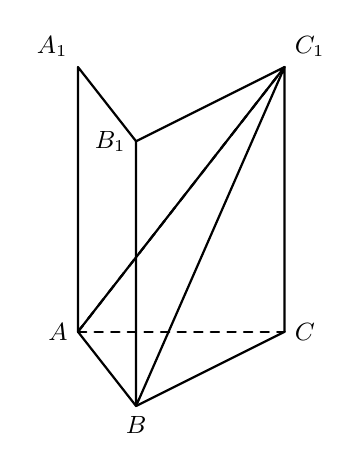
\begin{tikzpicture}[x=0.82cm,y=0.82cm,line cap=round,line join=round,line width=0.8pt,font=\small]
  \coordinate (A) at (0,0);
  \coordinate (B) at (0.9,-1.15);
  \coordinate (C) at (3.2,0);
  \coordinate (A1) at (0,4.1);
  \coordinate (B1) at (0.9,2.95);
  \coordinate (C1) at (3.2,4.1);
  \draw[dashed] (A)--(C);
  \draw[dashed] (A)--(C1);
  \draw (A)--(B)--(C);
  \draw (A)--(A1)--(B1)--(C1)--cycle;
  \draw (B)--(B1) (C)--(C1) (B)--(C1);
  \node[left] at (A) {$A$};
  \node[below] at (B) {$B$};
  \node[right] at (C) {$C$};
  \node[above left] at (A1) {$A_1$};
  \node[left] at (B1) {$B_1$};
  \node[above right] at (C1) {$C_1$};
\end{tikzpicture}
\end{center}
\nopagebreak[4]
\Needspace{4\baselineskip}
\textbf{解析}

设底面等边三角形高为 $h_0=\sqrt3/2$，棱柱高为 $H$。垂直于 $AB$ 的截面给出 $\cos60^\circ=h_0/\sqrt{h_0^2+H^2}$，所以 $H=3/2$。点 $C$ 到平面 $ABC_1$ 的距离为 $h_0H/\sqrt{h_0^2+H^2}=3/4$。

\gkanswer{答案：$3/4$。}

\end{answer}
\begin{answer}
\gksolhead{14}{}

\textbf{题目}：

若半径为1的圆分别与 $y$ 轴的正半轴和射线 $y=\frac{\sqrt3}{3}x\ (x\ge0)$ 相切，则这两个圆的方程为\gkblank{}。

\Needspace{4\baselineskip}
\textbf{解析}

本题保留未决。固定题面要求“这两个圆”。依指定射线切点需落在正半轴/射线上时，圆心条件目前只支持一个候选，无法从固定文本恢复第二个方程。答案记U；需同版勘误或可靠复本才能继续，不据推导猜改题干。

\gkanswer{答案：U（题面称“这两个圆”，但按同时与指定两条射线相切并要求切点位于射线上，当前条件只能确定一个候选；缺同版材料核查，不给出完整方程答案）。}

\end{answer}
\begin{answer}
\gksolhead{15}{}

\textbf{题目}：

某公司一年购买某种货物400吨，每次都购买 $x$ 吨，运费为4万元/次，一年的总存储费用为 $4x$ 万元，要使一年的总运费与总存储费用之和最小，则 $x=$\gkblank{}吨。

\Needspace{4\baselineskip}
\textbf{解析}

年购买次数为 $400/x$，费用和为 $1600/x+4x$。由均值不等式，其最小值在 $1600/x=4x$ 时取得，故 $x=20$吨。

\gkanswer{答案：20吨。}

\end{answer}
\begin{answer}
\gksolhead{16}{}

\textbf{题目}：

用数字0、1、2、3、4组成没有重复数字的五位数，则其中数字1、2相邻的偶数有\gkblank{}个。（用数字作答）

\Needspace{4\baselineskip}
\textbf{解析}

枚举五个数字的排列，要求首位非零、末位为偶数且1和2相邻，共24个。

\gkanswer{答案：24。}

\end{answer}
\begin{answer}
\gksolhead{17}{}

\textbf{题目}：

已知 $\tan\alpha+\cot\alpha=\frac52$，$\alpha\in(\frac\pi4,\frac\pi2)$，求 $\cos2\alpha$ 和 $\sin(2\alpha+\frac\pi4)$ 的值。

\Needspace{4\baselineskip}
\textbf{解析}

由 $\tan\alpha+\cot\alpha=2/\sin2\alpha=5/2$，得 $\sin2\alpha=4/5$。因 $\alpha\in(\pi/4,\pi/2)$，$\cos2\alpha<0$，故 $\cos2\alpha=-3/5$。再用正弦和角公式，$\sin(2\alpha+\pi/4)=1/(5\sqrt2)$。

\gkanswer{答案：$\cos2\alpha=-3/5$，$\sin(2\alpha+\pi/4)=1/(5\sqrt2)$。}

\end{answer}
\begin{answer}
\gksolhead{18}{}

\textbf{题目}：

甲、乙两台机床相互没有影响地生产某种产品，甲机床产品的正品率是0.9，乙机床产品的正品率是0.95。

（1） 从甲机床生产的产品中任取3件，求其中恰有2件正品的概率（用数字作答）；

（2） 从甲、乙两台机床生产的产品中各任取1件，求其中至少有1件正品的概率（用数字作答）。

\Needspace{4\baselineskip}
\textbf{解析}

\gksubpart{(1)}

所求概率为 $\binom32(0.9)^2(0.1)=0.243$。

\gksubpart{(2)}

用对立事件，至少一件正品的概率为 $1-(0.1)(0.05)=0.995$。

\gkanswer{答案（1）：0.243。}

\gkanswer{答案（2）：0.995。}

\end{answer}
\begin{answer}
\gksolhead{19}{}

\textbf{题目}：

如图，在五面体 $ABCDEF$ 中，点 $O$ 是矩形 $ABCD$ 的对角线的交点，面 $CDE$ 是等边三角形，棱 $EF\parallel BC$ 且 $EF=\frac12BC$。

（1） 证明：$FO\parallel$ 平面 $CDE$；

（2） 设 $BC=\sqrt3CD$，证明：$EO\perp$ 平面 $CDF$。
\nopagebreak[4]
\begin{center}% 2006 天津文科 Q19，源：固定 PDF 第 1 页（印刷页 338）。
% 节点：A,B,C,D 为矩形 ABCD 的角点，O 为对角线交点；E,F 为等边三角形 CDE
% 的第三顶点与棱端点。识别的实线：BC, CD, DE, EF, FB, EC, FC。
% 识别的虚线：AB, AD, AF, FO, EO, FD。题干说 O 是矩形 ABCD 对角线交点，
% 但源图未画 AC/BD 对角线，故未补画；O 是 FO 与 EO 两条虚线的端点。
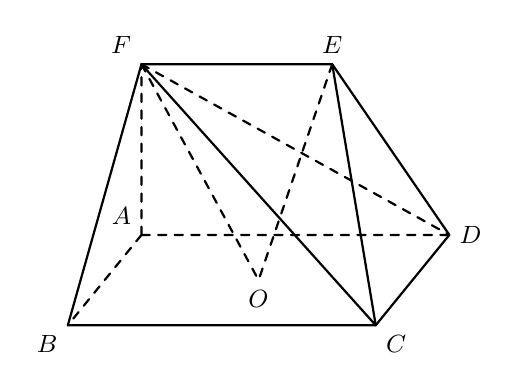
\begin{tikzpicture}[x=0.85cm,y=0.85cm,line cap=round,line join=round,line width=0.8pt,font=\small]
  \coordinate (A) at (1.1,1.35);
  \coordinate (B) at (0,0);
  \coordinate (C) at (4.6,0);
  \coordinate (D) at (5.7,1.35);
  \coordinate (O) at (2.85,0.675);
  \coordinate (F) at (1.1,3.9);
  \coordinate (E) at (3.95,3.9);
  % 隐藏棱与辅助虚线
  \draw[dashed] (A)--(B) (A)--(D) (A)--(F);
  \draw[dashed] (F)--(O) (E)--(O) (F)--(D);
  % 可见棱及内部实线
  \draw (B)--(C)--(D)--(E)--(F)--(B);
  \draw (E)--(C) (F)--(C);
  \node[above left] at (A) {$A$};
  \node[below left] at (B) {$B$};
  \node[below right] at (C) {$C$};
  \node[right] at (D) {$D$};
  \node[above] at (E) {$E$};
  \node[above left] at (F) {$F$};
  \node[below] at (O) {$O$};
\end{tikzpicture}
\end{center}
\nopagebreak[4]
\Needspace{4\baselineskip}
\textbf{解析}

\gksubpart{(1)}

取 $D=(0,0,0)$、$C=(s,0,0)$、$A=(0,0,t)$、$B=(s,0,t)$，则 $O=(s/2,0,t/2)$。令等边三角形第三顶点 $E=(s/2,\sqrt3s/2,0)$；由 $EF\parallel BC$ 且 $EF=BC/2$ 取 $F=(s/2,\sqrt3s/2,t/2)$。设 $M$ 为 $CD$ 中点，则 $FO=EM$，且 $EM$ 在平面 $CDE$ 内，因此 $FO\parallel$ 平面 $CDE$。

\gksubpart{(2)}

$BC=\sqrt3CD$ 给出 $t=\sqrt3s$。向量 $EO=(0,-\sqrt3s/2,t/2)$ 与 $DC=(s,0,0)$ 垂直；并且 $EO\cdot DF=-3s^2/4+t^2/4=0$。两条相交直线 $DC,DF$ 在平面 $CDF$ 内，故 $EO\perp$ 平面 $CDF$。

\gkanswer{答案（1）：见解析版}

\gkanswer{答案（2）：见解析版}

\end{answer}
\begin{answer}
\gksolhead{20}{}

\textbf{题目}：

已知函数 $f(x)=4x^3-3x^2\cos\theta+\frac1{32}$，其中 $x\in\mathbb R$，$\theta$ 为参数，且 $0\le\theta\le\frac\pi2$。

（1） 当 $\cos\theta=0$ 时，判断函数 $f(x)$ 是否有极值；

（2） 要使函数 $f(x)$ 的极小值大于零，求参数 $\theta$ 的取值范围；

（3） 若对（2） 中所求的取值范围内的任意参数 $\theta$，函数 $f(x)$ 在区间 $(2a-1,a)$ 内都是增函数，求实数 $a$ 的取值范围。

\Needspace{4\baselineskip}
\textbf{解析}

令 $c=\cos\theta$，则 $f'(x)=6x(2x-c)$。

\gksubpart{(1)}

$c=0$ 时 $f'(x)=12x^2\ge0$ 且不变号，函数无极值。

\gksubpart{(2)}

当 $c>0$ 时，局部极小点为 $x=c/2$，极小值 $f(c/2)=1/32-c^3/4$。要求它大于零等价于 $c<1/2$，故 $\theta\in(\pi/3,\pi/2]$。

\gksubpart{(3)}

对该参数范围，$0\le c<1/2$，导数为正的区间为 $x<0$ 或 $x>c/2$。区间 $(2a-1,a)$ 要对所有参数都为增区间，需完全落入左侧或统一落在右侧，即 $a\le0$ 或 $2a-1\ge1/4$。区间非空要求 $a<1$，所以 $a\in(-\infty,0]\cup[5/8,1)$。

\gkanswer{答案（1）：无极值。}

\gkanswer{答案（2）：$\theta\in(\pi/3,\pi/2]$。}

\gkanswer{答案（3）：$a\in(-\infty,0]\cup[5/8,1)$。}

\end{answer}
\begin{answer}
\gksolhead{21}{}

\textbf{题目}：

\Needspace{5\baselineskip}
已知数列 $\{x_n\}$ 满足 $x_1=x_2=1$，并且
\nopagebreak[4]
\[
\frac{x_{n+1}}{x_n}=\lambda\frac{x_n}{x_{n-1}}\quad(\lambda\text{为非零参数},\ n=2,3,4,\cdots)
\]

（1） 若 $x_1,x_3,x_5$ 成等比数列，求参数 $\lambda$ 的值；

\Needspace{5\baselineskip}
（2） 设 $0<\lambda<1$，常数 $k\in\mathbb N^*$ 且 $k\ge3$，证明：
\nopagebreak[4]
\[
\frac{x_{1+k}}{x_1}+\frac{x_{2+k}}{x_2}+\cdots+\frac{x_{n+k}}{x_n}<\frac{\lambda^k}{1-\lambda^k}\quad(n\in\mathbb N^*)
\]

\Needspace{4\baselineskip}
\textbf{解析}

令 $r_n=x_{n+1}/x_n$，则递推给出 $r_n=\lambda r_{n-1}$，且 $r_1=1$，所以 $x_n=\lambda^{(n-1)(n-2)/2}$。

\gksubpart{(1)}

$x_1,x_3,x_5$ 成等比数列等价于 $x_3^2=x_1x_5$，即 $\lambda^2=\lambda^6$。因 $\lambda\ne0$，得 $\lambda=\pm1$。

\gksubpart{(2)}

\Needspace{5\baselineskip}
对 $k\ge3$，$x_{i+k}/x_i=\lambda^{k(2i+k-3)/2}$。首项指数 $k(k-1)/2\ge k$，随后相邻指数相差 $k$。由于 $0<\lambda<1$，每项不大于对应的 $\lambda^{ki}$，所以
\nopagebreak[4]
\[
\sum_{i=1}^{n}\frac{x_{i+k}}{x_i}\le\sum_{i=1}^{n}\lambda^{ki}<\frac{\lambda^k}{1-\lambda^k}
\]

\gkanswer{答案（1）：$\lambda=\pm1$。}

\gkanswer{答案（2）：见解析版}

\end{answer}
\begin{answer}
\gksolhead{22}{}

\textbf{题目}：

如图，双曲线 $\frac{x^2}{a^2}-\frac{y^2}{b^2}=1\ (a>0,b>0)$ 的离心率为 $\frac{\sqrt5}2$，$F_1,F_2$ 分别为左、右焦点，$M$ 为左准线与渐近线在第二象限内的交点，且 $\overrightarrow{F_1M}\cdot\overrightarrow{F_2M}=-\frac14$。

（1） 求双曲线的方程；

（2） 设 $A(m,0)$ 和 $B(\frac1m,0)\ (0<m<1)$ 是 $x$ 轴上的两点。过点 $A$ 作斜率不为0的直线 $l$，使得 $l$ 交双曲线于 $C,D$ 两点，作直线 $BC$ 交双曲线于另一点 $E$。证明：直线 $DE$ 垂直于 $x$ 轴。
\nopagebreak[4]
\begin{center}% 2006 天津文科 Q22，源：固定 PDF 第 2 页（印刷页 339）。
% 几何比例依题面推出的 x^2-4y^2=1 作示意；以 m=3/4、参数 p=1/10 为一组
% 可行示例定位 A,B,C,D,E。拓扑：渐近线过 O；左准线过 M；DE 竖直；l 为 D-A-C，
% BC 为 E-C-B。其余焦点位置按 F1,F2=(±sqrt(5)/2,0)。
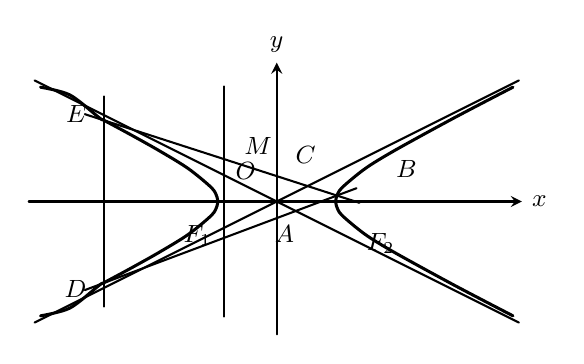
\begin{tikzpicture}[x=0.75cm,y=0.75cm,line cap=round,line join=round,line width=0.75pt,font=\small,>=stealth]
  % 坐标轴
  \draw[->] (-4.2,0)--(4.15,0) node[right] {$x$};
  \draw[->] (0,-2.25)--(0,2.35) node[above] {$y$};

  % 左准线 x=-2/sqrt(5)，及同一竖直线上的 D、E
  \draw (-0.894,-1.95)--(-0.894,1.95);
  \draw (-2.922,-1.78)--(-2.922,1.78);

  % 双曲线 x^2-4y^2=1
  \draw[line width=1.1pt] plot[smooth] coordinates {
    (-4,1.936) (-3.5,1.803) (-3,1.414) (-2.922,1.373)
    (-2.5,1.146) (-2,0.866) (-1.5,0.559) (-1.1,0.229)
    (-1.01,0.071) (-1,0)
  };
  \draw[line width=1.1pt] plot[smooth] coordinates {
    (-4,-1.936) (-3.5,-1.803) (-3,-1.414) (-2.922,-1.373)
    (-2.5,-1.146) (-2,-0.866) (-1.5,-0.559) (-1.1,-0.229)
    (-1.01,-0.071) (-1,0)
  };
  \draw[line width=1.1pt] plot[smooth] coordinates {
    (1,0) (1.01,0.071) (1.1,0.229) (1.5,0.559)
    (2,0.866) (3,1.414) (4,1.936)
  };
  \draw[line width=1.1pt] plot[smooth] coordinates {
    (1,0) (1.01,-0.071) (1.1,-0.229) (1.5,-0.559)
    (2,-0.866) (3,-1.414) (4,-1.936)
  };

  % 渐近线，以及 l=D-A-C、BC=E-C-B
  \draw (-4.1,2.05)--(4.1,-2.05);
  \draw (-4.1,-2.05)--(4.1,2.05);
  \draw (-3.25,-1.5)--(1.35,0.225);
  \draw (-3.25,1.479)--(1.4,-0.022);

  % 关键点（示意参数 m=3/4,p=1/10）
  \node[left] at (-3.05,1.48) {$E$};
  \node[left] at (-3.05,-1.48) {$D$};
  \node[above right] at (-0.72,0.62) {$M$};
  \node[below] at (-1.34,-0.24) {$F_1$};
  \node[above left] at (-0.18,0.20) {$O$};
  \node[below left,xshift=-6pt,yshift=-5pt] at (0.75,0) {$A$};
  \node[above left,xshift=-4pt,yshift=8pt] at (1.02,0.101) {$C$};
  \node[below right,xshift=5pt,yshift=-8pt] at (1.118,0) {$F_2$};
  \node[above right,xshift=11pt,yshift=5pt] at (1.333,0) {$B$};
\end{tikzpicture}
\end{center}
\nopagebreak[4]
\Needspace{4\baselineskip}
\textbf{解析}

\gksubpart{(1)}

离心率给出 $c/a=\sqrt5/2$，于是 $b^2/a^2=1/4$。左准线和第二象限渐近线交点为 $M=(-2a/\sqrt5,a/\sqrt5)$。利用 $\overrightarrow{F_1M}\cdot\overrightarrow{F_2M}=|M|^2-c^2=-a^2/4=-1/4$ 得 $a=1$，$b=1/2$，双曲线方程为 $x^2-4y^2=1$。

\gksubpart{(2)}

令 $P(u)=((1+u^2)/(1-u^2),u/(1-u^2))$ 参数化 $x^2-4y^2=1$，设 $C=P(p),D=P(q)$。由 $A,C,D$ 共线可得 $pq=(1-m)/(1+m)=r$。由双曲线上参数弦的斜率公式，$BC$ 与弦 $CP(-q)$ 的斜率同为 $mp/((m+1)(p^2-r))$，所以直线 $BC$ 的另一交点为 $E=P(-q)$。而 $P(q)$ 与 $P(-q)$ 横坐标相同，故 $x_D=x_E$，即 $DE\perp x$轴。此证明对应题设中两个不同交点的非退化情形。

\gkanswer{答案（1）：$x^2-4y^2=1$。}

\gkanswer{答案（2）：见解析版}

\end{answer}